%%----------------------------------------------------------------------
%%----------------------------------------------------------------------
\clearpage
\pagetitle{Organization}

\begin{columns}

This section describes how to conduct a \emph{Legacies} campaign, and
is mostly intended for the organizer.

\missionheading{Schedule}

Recon Squad games can be easily run in about~60 minutes in an event
setting with boards pre-arranged and armies unpacked before the clock
starts for each round.  Generally matches take at most~90 minutes even
at a very casual pace with no preparation beforehand.  The Cataclysm
game can be comfortably played in~4 hours including setup.  It's
therefore feasible to run \emph{Legacies} over either several
evenings, or a single full day.  A sample schedule for a single-day is:

\bigskip
\centerline{\begin{tabular}{cl}
11:00	 	& Doors open\\
11:50	 	& Registration Closes\\
12:00	 	& Campaign Briefing \& Alliance Pairings\\
12:15	 	& Round 1\\
1:25	 	& Alliance Pairings\\
1:35	 	& Round 2\\
2:40	 	& Alliance Pairings\\
2:50	 	& Round 3\\
3:50	 	& Alliance Pairings\\
4:00	 	& Round 4\\
5:00	 	& Dinner Break\\
5:30	 	& The Cataclysm\\
9:30	 	& Campaign Outcome \& Prizes\\
\end{tabular}}

\vfill

\noindent\fbox{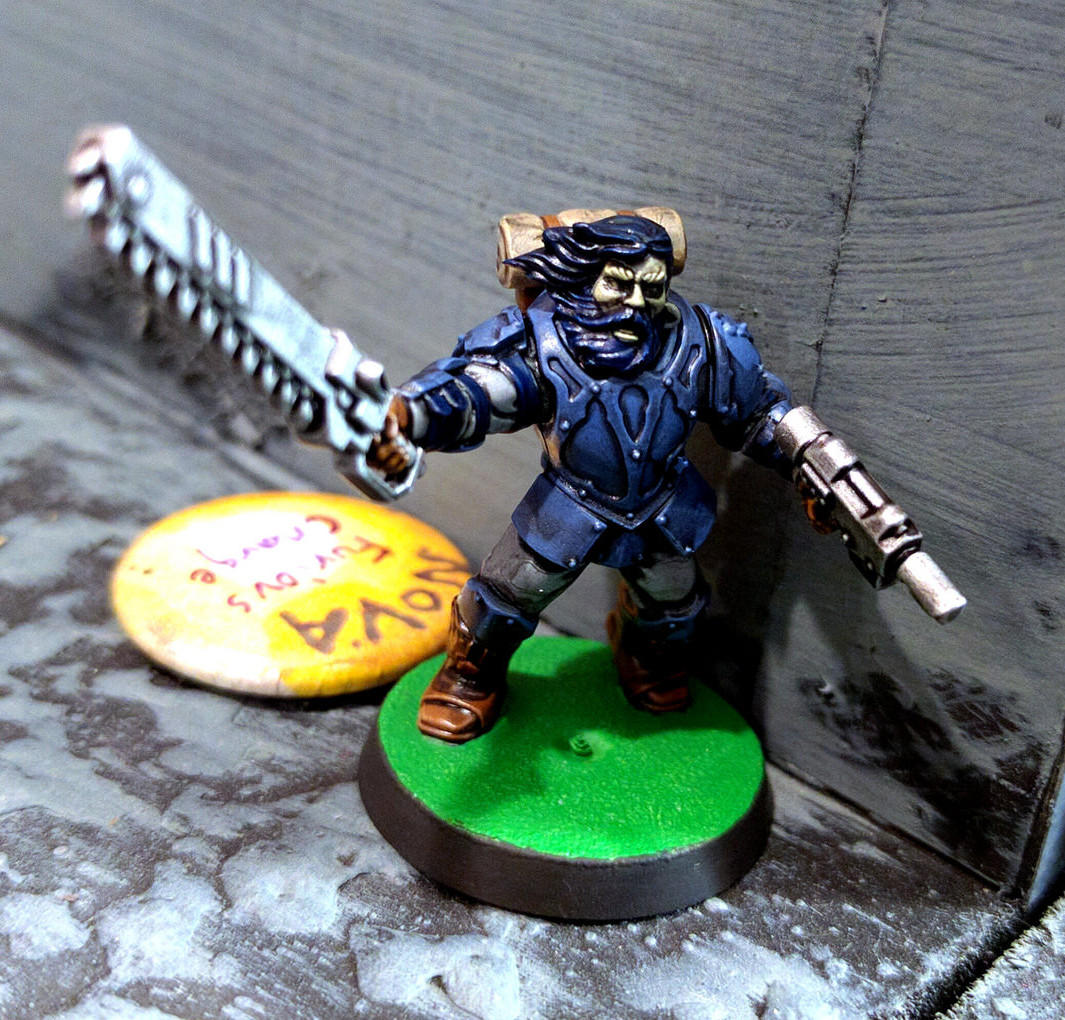
\includegraphics[width=\linewidth]{images/renegade-sgt-cropped.jpg}}

\columnbreak%

\missionheading{Alliances \& Story}

At the start of the campaign, the players are organized into two
alliances with an equal number of players.  In some groups this might
be faction specific, e.g., Chaos Daemons versus Eldar.  Generally
though an alliance will be comprised of several factions and can be
given a less specific title such as the Forces of Order, Legions of
Discord, or the Spoiler Horde.  How players are assigned alliances is
up to the organizer.  In a large event with mostly strangers and
tournament leanings it might be simply random.  In more
narrative-oriented and casual settings though, some attempt should be
made to take into account thematic cohesiveness as well as balanced
skill levels.

The concept behind the campaign is that each recon squad is a team of
veterans or other distinguished warriors tasked with several special
operations as part of a larger battle or war.  In the course of those
missions their paths eventually all cross, resulting in the larger
final battle.  Any specific background story is up to the organizer
and players, enabling a range of narratives with more or less detail.

\missionheading{Setup}

In advance of the campaign, players should be pointed to the Recon
Squad rules and the Missions section of this packet so they can design
their Recon Squad and Cataclysm army lists.  The campaign is themed
around players fielding a single Recon Squad list throughout, but the
organizer should feel free to be flexible about that requirement if
they wish.  In a campaign run over multiple days there is no need to
require Cataclysm lists be finalized until the last event.

Preparing for the campaign is very simple.  For each of the two
alliances, print and cut apart enough sets of the~8 legacy cards in
the Missions section to have at least one card per player.
Also print and cut apart enough sets of the~8 mission sheets to have
one for each match.  For a campaign with up to~16 players this means
making two sets of legacy cards and one set of mission sheets.

With anything but a very small number of players, it's probably easier
to have players record results separately from the mission sheets,
especially as the latter might be used multiple times.  In that case,
print and cut apart enough copies of the scorecards at the end of this
section to have one for each match.  Finally, if using the scoring
mechanism described here, also print and cut apart enough copies of
the ballots and tickets from the end of this section to have one
painting ballot per player and as many sportsmanship tickets as you
think might be necessary.

\missionheading{Legacies}

After being assigned an alliance, each player chooses a legacy.  No
legacy may be selected twice within an alliance until all legacies
have been chosen at least once, and so on if there are even more
players.  Otherwise the alliance members may discuss among themselves
how to divy up the legacies.  If there is any contention, either ask
the players in random order to choose, or randomly assign legacies.

Each legacy lists three Recon Squad Missions and gives a Cataclysm
Objective and Legacy Bonus.  To achieve their legacy, players must
accomplish the Cataclysm Objective in the final team battle.  If they
win at least two of the three Recon Squad Missions in the given role
of attacker, defender, or either, then they receive their Legacy Bonus
in the Cataclysm.

Players' chosen legacies, match results, and whether or not they are
succeeding at their missions are all public information throughout the
campaign.

\missionheading{Round Pairings}

Recon Squad match pairings are made strategically by the alliances to
help their players achieve their legacy missions and further their
collective strategic goals.  Before each round, the alliances
alternate nominating one of their remaining unpaired players along
with a mission and role (attacker or defender).  The opposing alliance
then responds with a player for the match, who takes the other mission
role and chooses an unclaimed game board to play on.  This player must
be in the same or best similar win/draw/loss bracket as the nominated
player, unless the number of players is not great enough to make this
restriction without repeating match pairings.  In that case the later
rounds might require specific pairings to not have repeats.

For the first round, the initial alliance to put a player forward is
determined either randomly or based on the background story or the
outcomes of connected preceding events.  In subsequent rounds the
alliances alternate making the initial nomination.

Players should use the checkboxes on their legacy cards to record
victories toward the Recon Squad Mission requirements, in addition to
the organizer keeping track.  It does not matter if the player was
nominated or the responding opponent, and they do not have to complete
the missions in any order.  In order to get their Legacy Bonus in the
Cataclysm they simply have to win each mission in the required role at
some point in the campaign.  Similarly, a player can attempt a mission
and role pair multiple times.  However, no advantage is gained by
winning the same mission and role pair multiple times.

\missionheading{Cataclysm}

Following the four rounds of Recon Squad games, the campaign concludes
by pitching the two teams against each other directly in the
Cataclysm.  Each player essentially adds 300 points to their Recon
Squad, as described in detail in the Missions section.  The board for
the Cataclysm game should be~4' wide as usual, and roughly as many
feet long as there are players in the campaign.  So an~8-player
campaign would conclude on an 8'x4' table.  One idea to consider is
simply moving together boards used in the Recon Squad rounds, so that
the battle thematically continues directly over the same terrain.

%An important role for the organizer in the Cataclysm is keeping time.
%A schedule must be established

\missionheading{Scoring and Prizes}

\emph{Legacies} is oriented to casual play.  However, it can easily be
used for a narrative tournament format.  Any prizes should be small
and fairly well distributed though to limit the stakes, given that top
players may not face each other if they're in the same alliance,
players don't all contest the same scenarios, some missions are
asymmetric, and so on.  There should also perhaps be two sets of
prizes for any gameplay awards, one for each alliance.  The following
is one potential scoring and prize scheme, but the organizer should of
course feel free to devise their own.

\missionsubheading{Prizes.} The following prizes are offered:

\begin{itemize}\shortlist
\item Overall alliance winners based on total scores;
\item Painting and hobby based on player voting;
\item Best general, based on battle points earned.
\end{itemize}

\missionsubheading{Overall Scores.} A total of~100 points are
available for each player throughout the campaign:

\begin{itemize}\shortlist
\item 60 points for game results;
\item 20 points for painting and hobby;
\item 20 points for sportsmanship.
\end{itemize}

\missionsubheading{Game Results.} 

Each of the four Recon Squad missions are worth up to~12 points:
\begin{itemize}\shortlist
\item Major victories award~10 points to the winner and 0 to the not-winner;
\item Minor victories award~7 points to the winner and 3 to the not-winner;
\item Draws award~5 points to both players.
\item 2 bonus points are available in each mission.
\end{itemize}

Players may also earn up to~12 points in the Cataclysm toward their
individual game results:
\begin{itemize}\shortlist
\item 7 points for winning their Cataclysm Objective;
\item 3 points if they earned their Legacy Bonus;
\item 2 points if their alliance won the Cataclysm.
\end{itemize}


\missionsubheading{Painting and Hobby Scores.} 

Painting and hobby work is scored objectively by the organizer
applying this rubric to the entire army:

\begin{itemize}\shortlist
\item All models assembled and primed: +5 pts
\item All models three-color minimum: +5 pts
\item All models based (paint/flock): +4 pts
\item Advanced painting techniques present on any model (washes,
  drybrushing, etc.): +3 pts
\item Advanced basing techniques present on any model (3D details,
  varied flock, etc.): +3 pts
\end{itemize}

Note that this goes solely toward overall scores.  The painting prize
is based purely on player voting.

\missionsubheading{Sportsmanship.}

By default, a player earns~5 points for sportsmanship in each Recon
Squad round.  However, if their opponent submits a sportsmanship
ticket then they are docked points for any poor behavior:

\begin{itemize}\shortlist
\item Openly hostile or rude: -3 pts
\item Unnecessarily competitive in army, list, or attitude: -2 pts
\item Sloppy with measuring, moving, line of sight, or dice: -2 pts
\item Unreasonably late, overly slow playing, or too inattentive: -1 pt
\item Significantly unfamiliar with rules or made too many mistakes:
  -1 pt
\item Not prepared with clear, typed army lists: -1 pt
\end{itemize}

Hopefully few or none of these tickets need to be submitted; it's
perfectly acceptable for players to not find any reason to penalize
their opponents.  It should be feasible then to give each player one
at the start of the campaign and only give out more as needed.

\missionsubheading{Painting Award.}  Separate from the overall scores,
a painting and craftsmanship prize is awarded based on player voting.
Each player must submit a ballot ranking what they consider the best
army among all those in the campaign.  Players may not vote for
themselves.  For each ballot, the top army receives~3 votes, the
second~2 votes, and the third~1 vote.  The army with the most votes
wins the prize.

\end{columns}

\squelchbackground
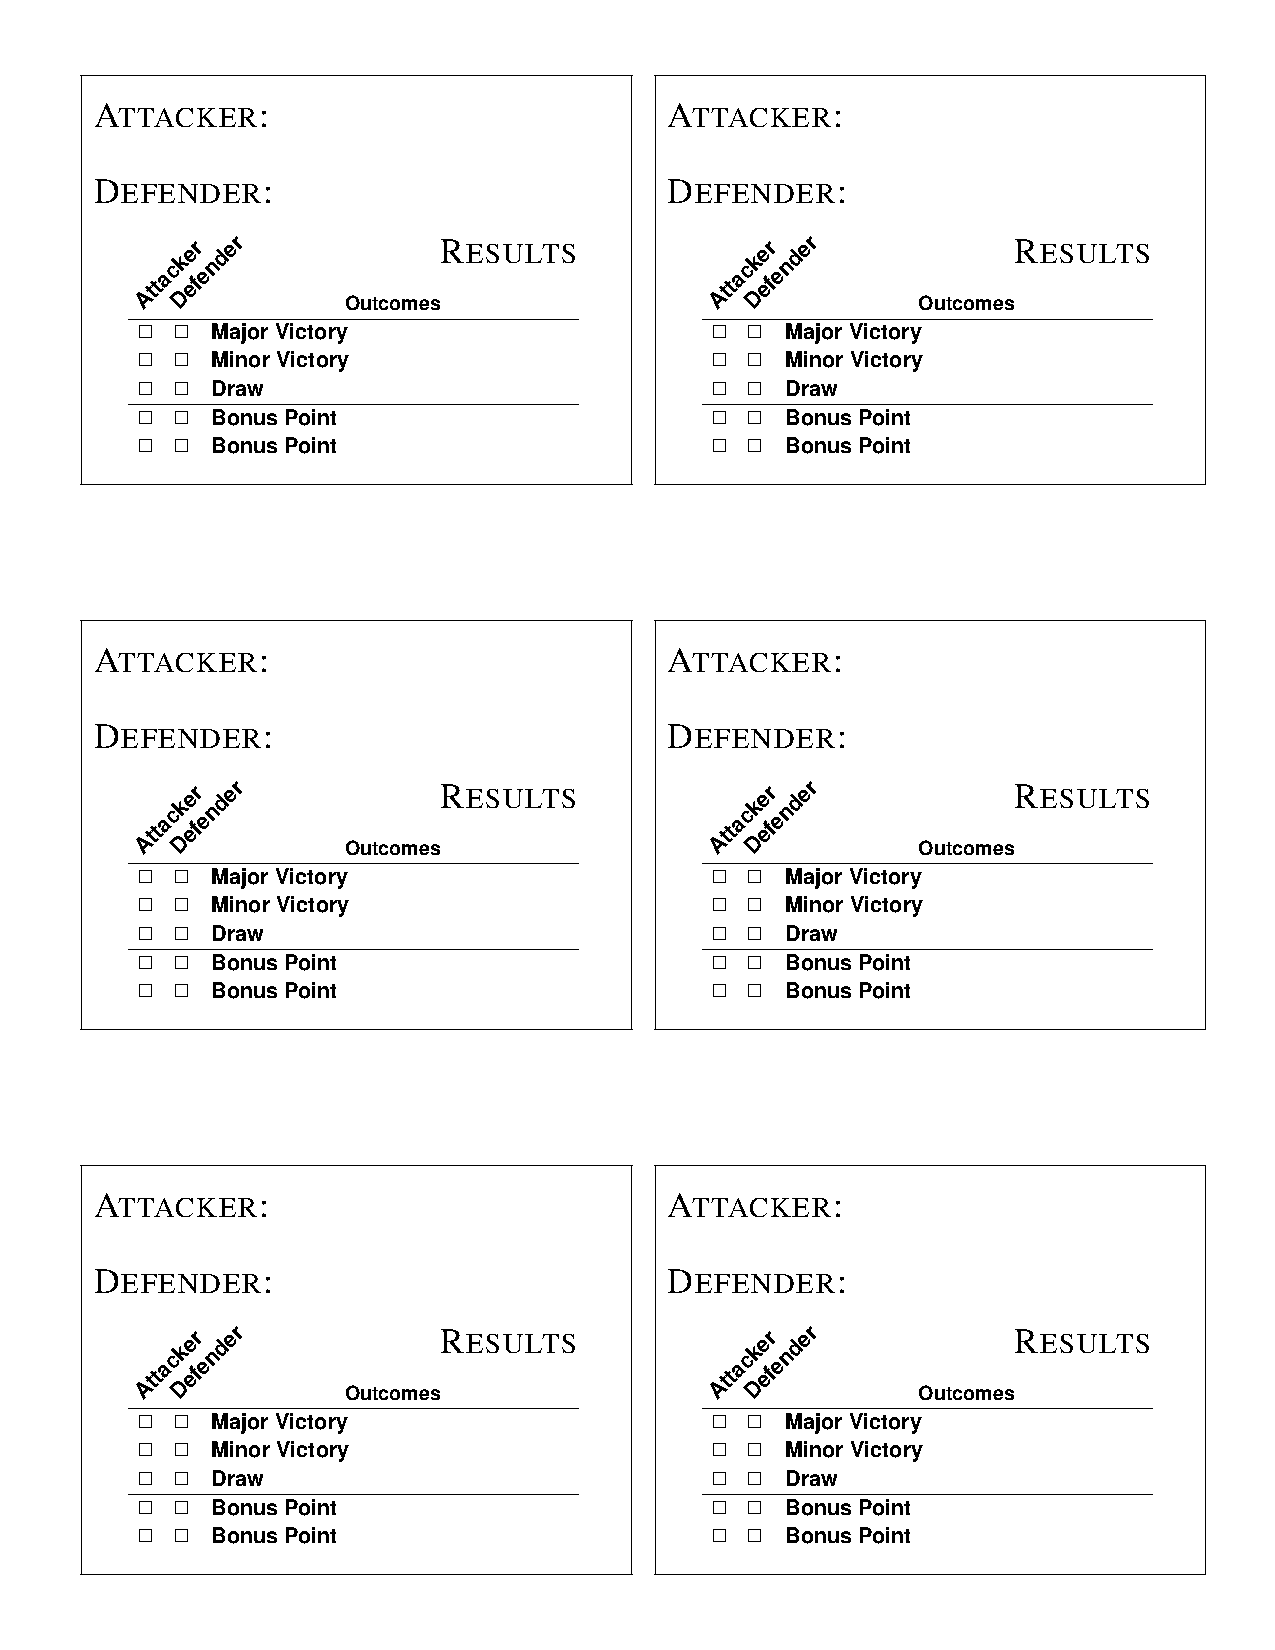
\includepdf[pages={1}]{20141220-scorecards.pdf}
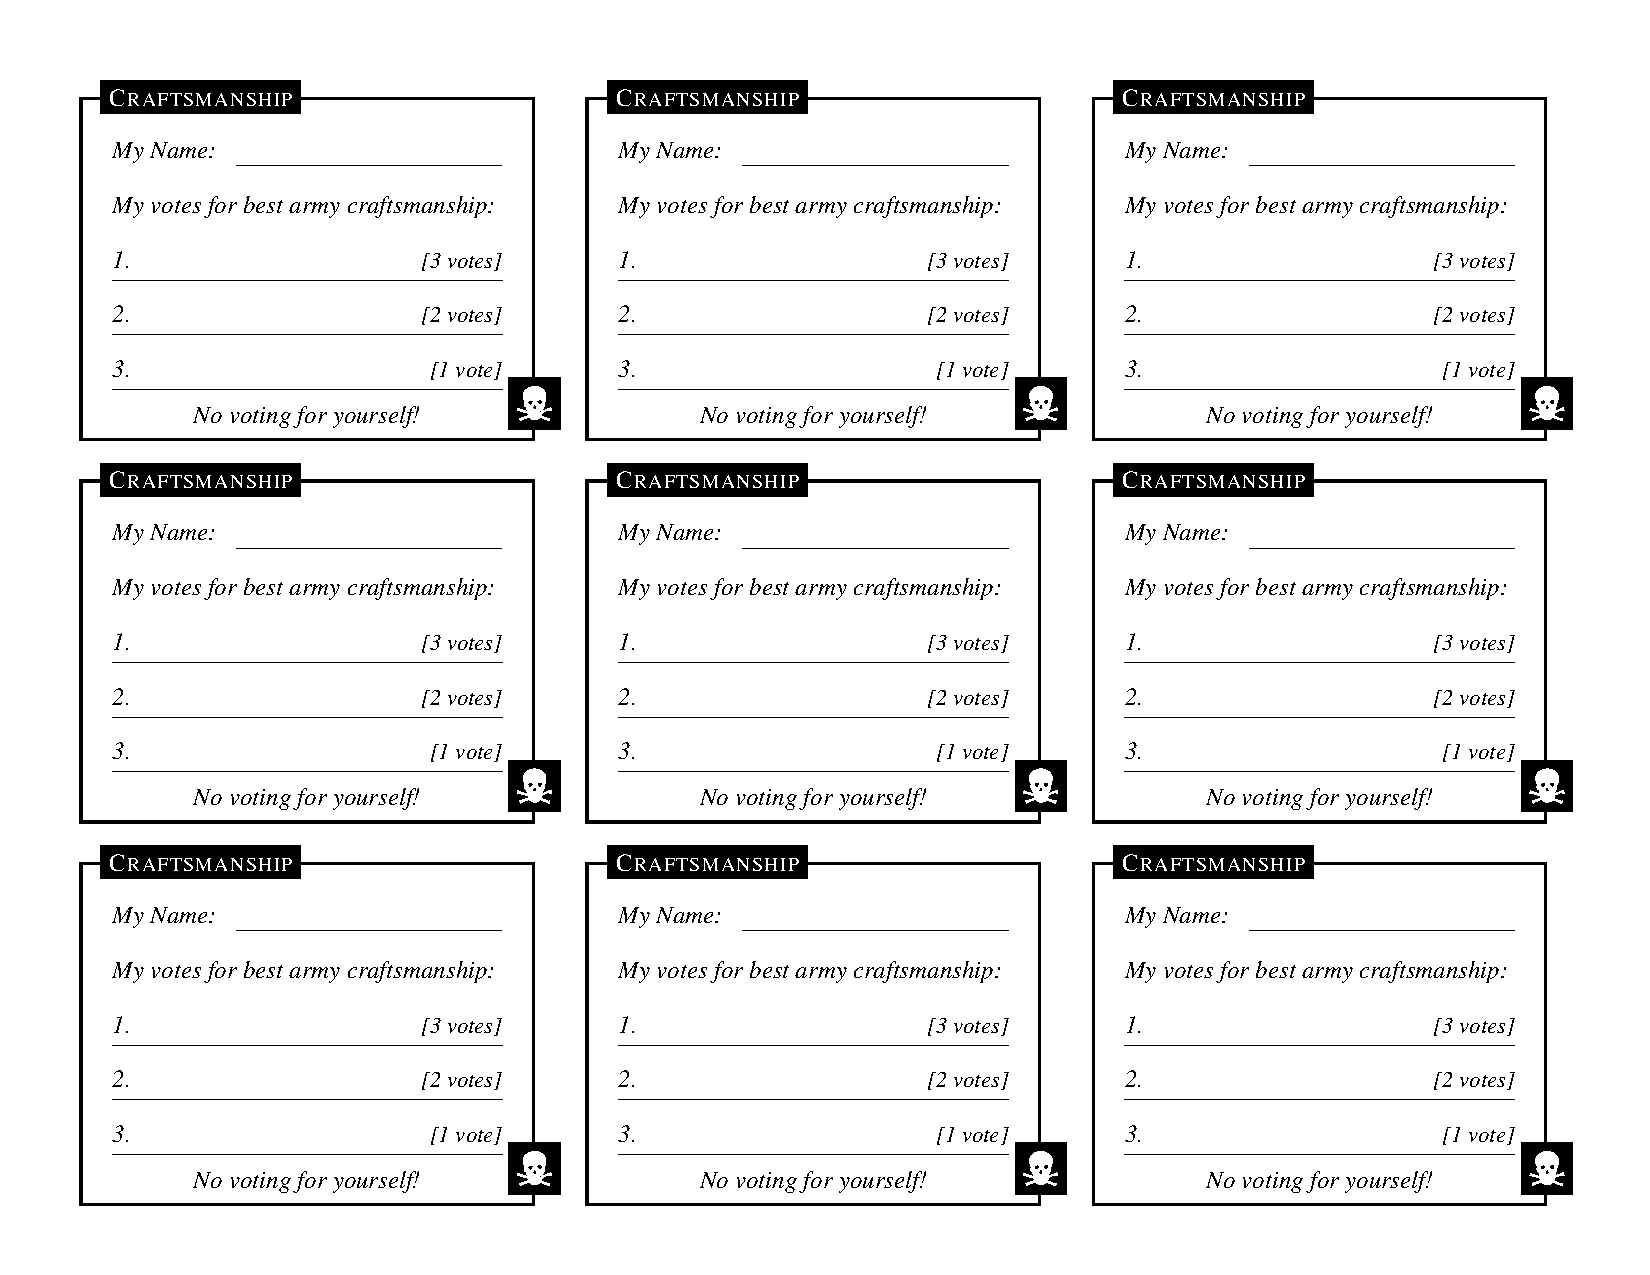
\includepdf[pages={1},landscape=true]{2016-painting.pdf}
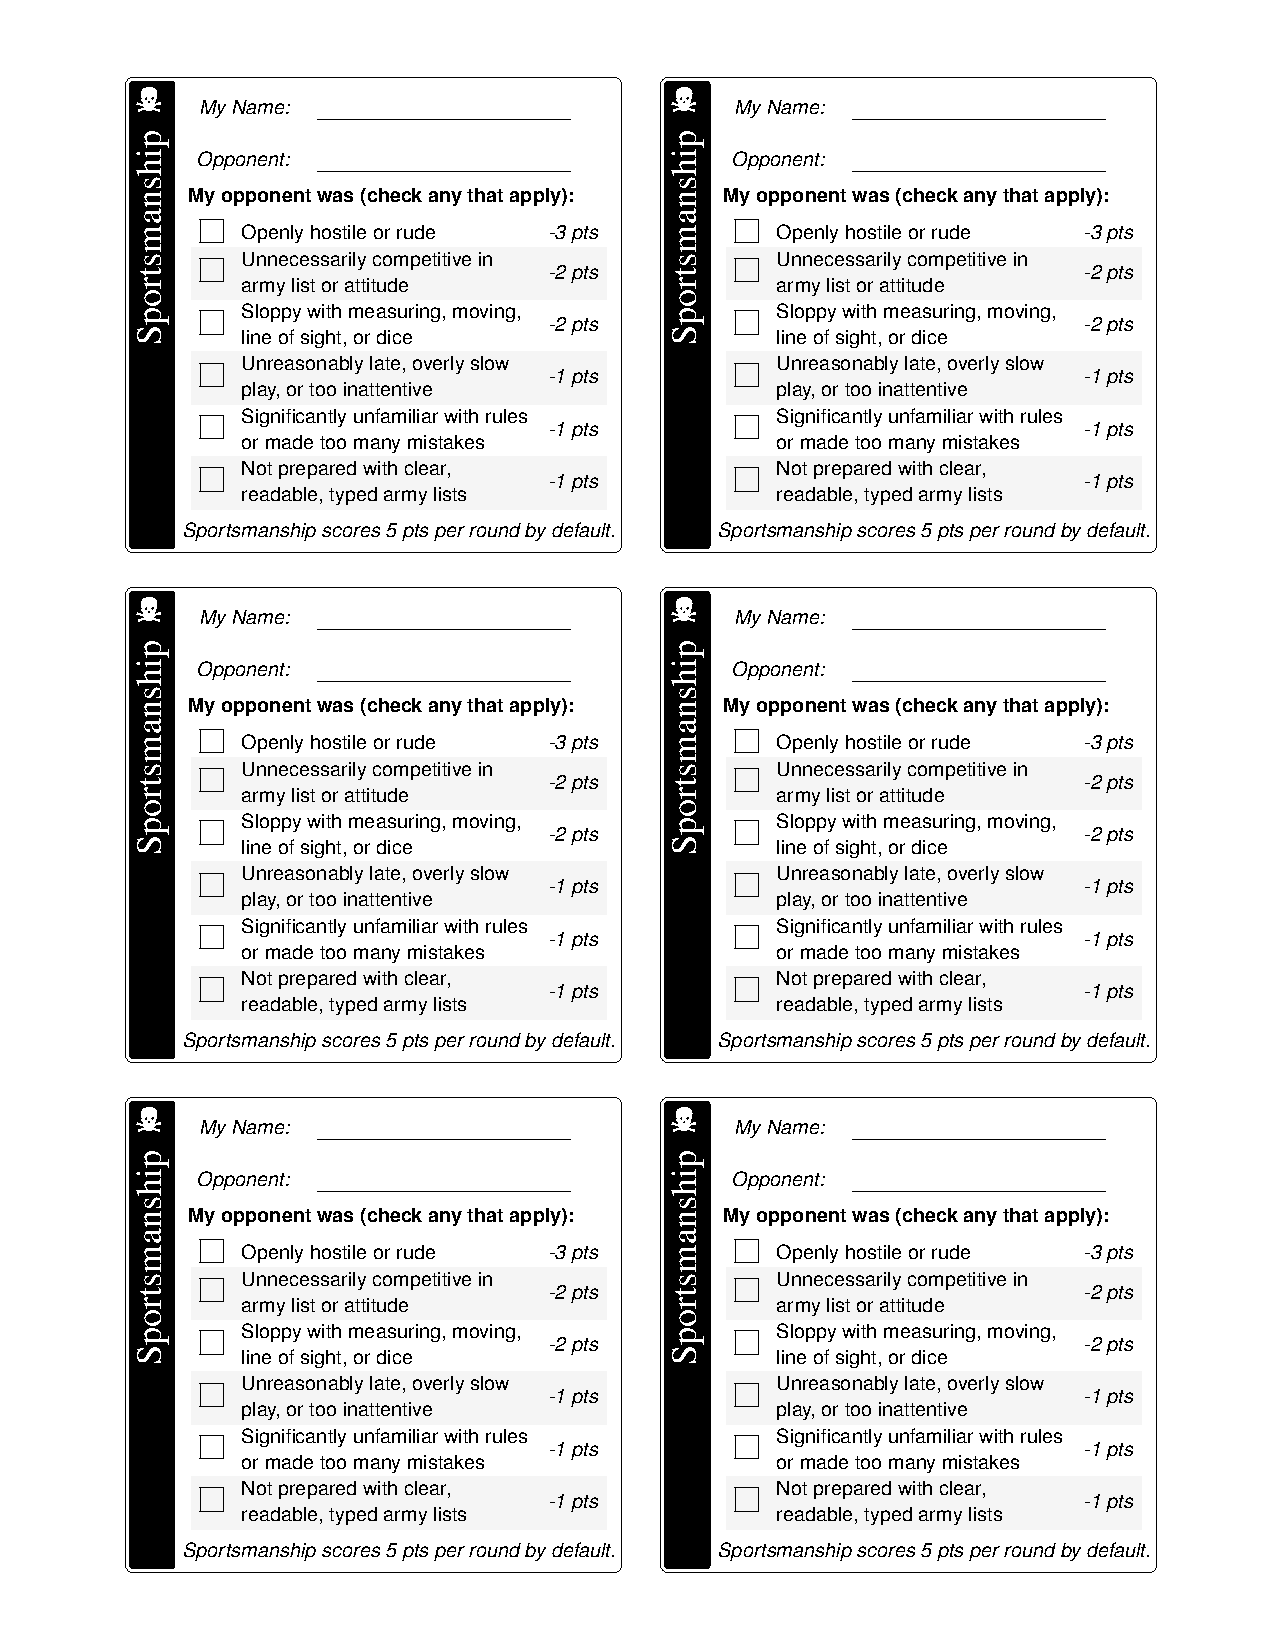
\includepdf[pages={1}]{2016-sportsmanship.pdf}
\restorebackground
